% Компіляція: lualatex -shell-escape report.tex (двічі)
\documentclass[12pt,a4paper]{article}

\usepackage{fontspec}
\usepackage{polyglossia}
\setdefaultlanguage{ukrainian}
\setmainfont{NewComputerModern10}
\setsansfont{Noto Sans}
\setmonofont{Noto Sans Mono}[
  Scale=0.82,
  ItalicFont={Noto Sans Mono},
  ItalicFeatures={FakeSlant=0.2}
]

\usepackage{
  amsmath,
  amssymb,
  array,
  booktabs,
  caption,
  enumitem,
  float,
  geometry,
  graphicx,
  microtype,
  titlesec,
  xcolor
}
\geometry{left=2cm,right=2cm,top=2cm,bottom=2cm}
\setlength{\parindent}{1.25cm}
\setlength{\parskip}{0pt}
\linespread{1.08}
\titleformat{\section}
  {\normalfont\fontsize{14}{16}\selectfont\bfseries}
  {\thesection}{0.6em}{}
\titleformat{\subsection}
  {\normalfont\fontsize{12}{14}\selectfont\bfseries}
  {\thesubsection}{0.6em}{}
\titlespacing*{\section}{0pt}{1.4em}{0.65em}
\titlespacing*{\subsection}{0pt}{1.1em}{0.45em}
\captionsetup{font=small,labelfont=bf,labelsep=endash}
\captionsetup[table]{position=bottom,skip=5pt}

\usepackage[newfloat]{minted}
\SetupFloatingEnvironment{listing}{name=Лістинг}
\setminted{%
  fontsize=\scriptsize,
  linenos,
  breaklines,
  breakanywhere,
  autogobble,
  frame=single,
  framesep=2mm,
  bgcolor=gray!5,
  tabsize=4
}

\usepackage[
  unicode,
  colorlinks=true,
  linkcolor=black,
  urlcolor=blue,
  pdftitle={ІО-41, Давидчук Артем, Вступ до штучного інтелекту, Лабораторна робота №1},
  pdfauthor={Давидчук Артем},
  pdfsubject={Ознайомлення з середовищем Jupyter Notebook}
]{hyperref}

\begin{document}

\pagenumbering{gobble}
\begin{titlepage}
  \begin{center}
    
\includegraphics[width=0.7\textwidth]{../../../../../../templates/letterhead.png}
  \end{center}

  \begin{center}
    \large
    Національний технічний університет України\\
    «Київський політехнічний інститут імені Ігоря Сікорського»\\[1em]
    Факультет інформатики та обчислювальної техніки\\
    Кафедра обчислювальної техніки
  \end{center}

  \vfill

  \begin{center}
    \textbf{\LARGE Вступ до штучного інтелекту}\\[2em]
    \textbf{\Large Лабораторна робота №1}\\[0.7em]
    \parbox{0.9\textwidth}{\centering
      «Ознайомлення з середовищем Jupyter Notebook»}
  \end{center}

  \vfill

  \begin{flushright}
    \begin{minipage}{0.48\textwidth}
      Виконав: студент групи ІО-41\\
      \textit{Давидчук Артем}\\[1em]
      Перевірив: \textit{Кочура Ю. П.}
    \end{minipage}
  \end{flushright}

  \vfill

  \begin{center}Київ --- 2026\end{center}
\end{titlepage}
\pagenumbering{arabic}

\section{Мета роботи}

Підготувати оточення для виконання подальших лабораторних робіт з
дисципліни «Вступ до штучного інтелекту».

\section{Завдання}

Необхідно створити графову топологію комп'ютерної мережі у формі квадратної
решітки, призначити ребрам ваги, що відповідають затримці, видалити задану
кількість ребер зі збереженням зв'язності графа та візуалізувати початковий і
результуючий графи.

\section{Опис алгоритму}

Мережа подається неорієнтованим зваженим графом \(G=(V,E)\), де \(V\) ---
множина вузлів, а \(E\) --- множина каналів зв'язку. Вузли всередині програми
представлені кортежами \texttt{(row, column)}. Для
\(\texttt{nodes\_num}=k^2\) створюється квадратна решітка розміру
\(k\times k\). Ребра додаються лише між горизонтальними та вертикальними
сусідами: для кожного вузла перевіряються сусід униз і сусід праворуч. Завдяки
використанню \texttt{nx.Graph} отриманий граф є неорієнтованим, а ребра не
дублюються.

Кожне ребро отримує випадкову цілу вагу в заданому діапазоні. Нижню та верхню
межі визначають параметри \texttt{min\_weight} і \texttt{max\_weight}
відповідно. Ця вага моделює затримку передавання даних у мілісекундах. Кожному
вузлу призначається унікальна адреса за його позицією:
\texttt{10.0.<row>.<column>}.

Перед видаленням список ребер випадково перемішується. Чергове ребро тимчасово
видаляється, а функція \texttt{nx.is\_connected(graph)} перевіряє зв'язність
графа. Якщо зв'язність втрачено, ребро відновлюється з початковою вагою. Якщо
граф залишається зв'язним, видалення зараховується. Процес триває, доки не
буде видалено задану кількість ребер.

Квадратна решітка має \(|V|=k^2\) вузлів та \(|E|=2k(k-1)\) ребер.
Максимальна кількість ребер, яку можна видалити зі збереженням зв'язності,
дорівнює
\begin{equation}
  m_{\max}=|E|-|V|+1
  =2k(k-1)-k^2+1
  =(k-1)^2.
\end{equation}
У програмі використано саме послідовне видалення з перевіркою та можливим
відновленням ребра.

\section{Програмний код}

Нижче наведено код із виконаного файлу \texttt{lab1.ipynb} без службових
метаданих формату Jupyter Notebook.

\subsection{Імпорт бібліотек}

\begin{listing}[H]
\begin{minted}{python}
import math
import random

import matplotlib.pyplot as plt
import networkx as nx
\end{minted}
\caption{Імпорт використаних бібліотек}
\end{listing}

\subsection{Перевірка параметрів}

\begin{listing}[H]
\begin{minted}{python}
def validate_args(nodes_num, edges_to_delete, min_weight, max_weight):
    k = math.isqrt(nodes_num)
    if k * k != nodes_num:
        raise ValueError("nodes_num must be a perfect square")
    max_edges_to_delete = (k - 1) ** 2

    if edges_to_delete < 0 or edges_to_delete > max_edges_to_delete:
        raise ValueError(f"edges_to_delete must be between 0 and {max_edges_to_delete}")

    if min_weight <= 0 or min_weight > max_weight:
        raise ValueError("invalid weight range")

    print("Arguments validated")
\end{minted}
\caption{Функція перевірки вхідних параметрів}
\end{listing}

\subsection{Створення графа}

\begin{listing}[H]
\begin{minted}{python}
def create_graph(nodes_num=25, min_weight=1, max_weight=10):
    k = math.isqrt(nodes_num)
    nodes = []
    edges = []
    for i in range(k):
        for j in range(k):
            nodes.append((i, j))

    for node in nodes:
        i, j = node
        if i + 1 < k:
            weight = random.randint(min_weight, max_weight)
            edges.append(
                (
                    node,
                    (i + 1, j),
                    weight
                )
            )

        if j + 1 < k:
            weight = random.randint(min_weight, max_weight)
            edges.append(
                (
                    node,
                    (i, j + 1),
                    weight
                )
            )

    graph = nx.Graph()

    for node in nodes:
        graph.add_node(
            node,
            address=f"10.0.{node[0]}.{node[1]}"
        )

    for u, v, weight in edges:
        graph.add_edge(u, v, weight=weight)

    print("Graph successfully created")

    return graph
\end{minted}
\caption{Функція створення квадратного зваженого графа}
\end{listing}

\subsection{Візуалізація графа}

\begin{listing}[H]
\begin{minted}{python}
def show_graph(graph):

    pos = {}
    labels = {}

    for node in graph.nodes():
        i, j = node
        pos[node] = (j, -i)

    for node in graph.nodes():
        labels[node] = graph.nodes[node]["address"]

    plt.figure(figsize=(10, 8))

    nx.draw(
        graph,
        pos,
        labels=labels,
        with_labels=True,
        node_size=1600,
        font_size=8
    )

    edge_labels = nx.get_edge_attributes(
        graph,
        "weight"
    )

    nx.draw_networkx_edge_labels(
        graph,
        pos,
        edge_labels=edge_labels,
        font_size=8
    )

    plt.show()
\end{minted}
\caption{Функція візуалізації графа}
\end{listing}

\subsection{Видалення ребер}

\begin{listing}[H]
\begin{minted}{python}
def remove_edges(graph, m):

    edges = list(graph.edges())
    random.shuffle(edges)

    removed = 0

    while removed < m:

        edge = edges.pop()
        edge_weight = graph[edge[0]][edge[1]]["weight"]

        graph.remove_edge(edge[0], edge[1])

        if nx.is_connected(graph):
            removed += 1
        else:
            graph.add_edge(edge[0], edge[1], weight=edge_weight)

    print(f"Successfully deleted {m} edges")
\end{minted}
\caption{Функція видалення ребер зі збереженням зв'язності}
\end{listing}

\subsection{Параметри та виконання}

\begin{listing}[H]
\begin{minted}{python}
nodes_num = 25
edges_to_delete = 6
min_weight = 1
max_weight = 10

validate_args(nodes_num, edges_to_delete, min_weight, max_weight)

graph = create_graph(nodes_num, min_weight, max_weight)
initial_edges = graph.number_of_edges()
show_graph(graph)

remove_edges(graph, edges_to_delete)
show_graph(graph)

expected_edges = initial_edges - edges_to_delete
is_connected = nx.is_connected(graph)

assert graph.number_of_edges() == expected_edges
assert is_connected

print(f"Кількість вузлів: {graph.number_of_nodes()}")
print(f"Кількість ребер: {graph.number_of_edges()}")
print(f"Граф зв’язний: {is_connected}")
\end{minted}
\caption{Параметри генерації, виконання та підсумкова перевірка}
\end{listing}

\section{Результати виконання}

Для запуску використано параметри, наведені в табл.~\ref{tab:parameters}.

\begin{table}[H]
  \centering
  \renewcommand{\arraystretch}{1.18}
  \begin{tabular}{|l|c|}
    \hline
    \textbf{Параметр} & \textbf{Значення} \\
    \hline
    \texttt{nodes\_num} & 25 \\ \hline
    \texttt{edges\_to\_delete} & 6 \\ \hline
    \texttt{min\_weight} & 1 \\ \hline
    \texttt{max\_weight} & 10 \\ \hline
  \end{tabular}
  \caption{Параметри виконання програми}
  \label{tab:parameters}
\end{table}

Початкова топологія містить 25 вузлів і 40 ребер. Адреси вузлів та випадково
згенеровані ваги ребер відображено на рис.~\ref{fig:initial-topology}.

\begin{figure}[H]
  \centering
  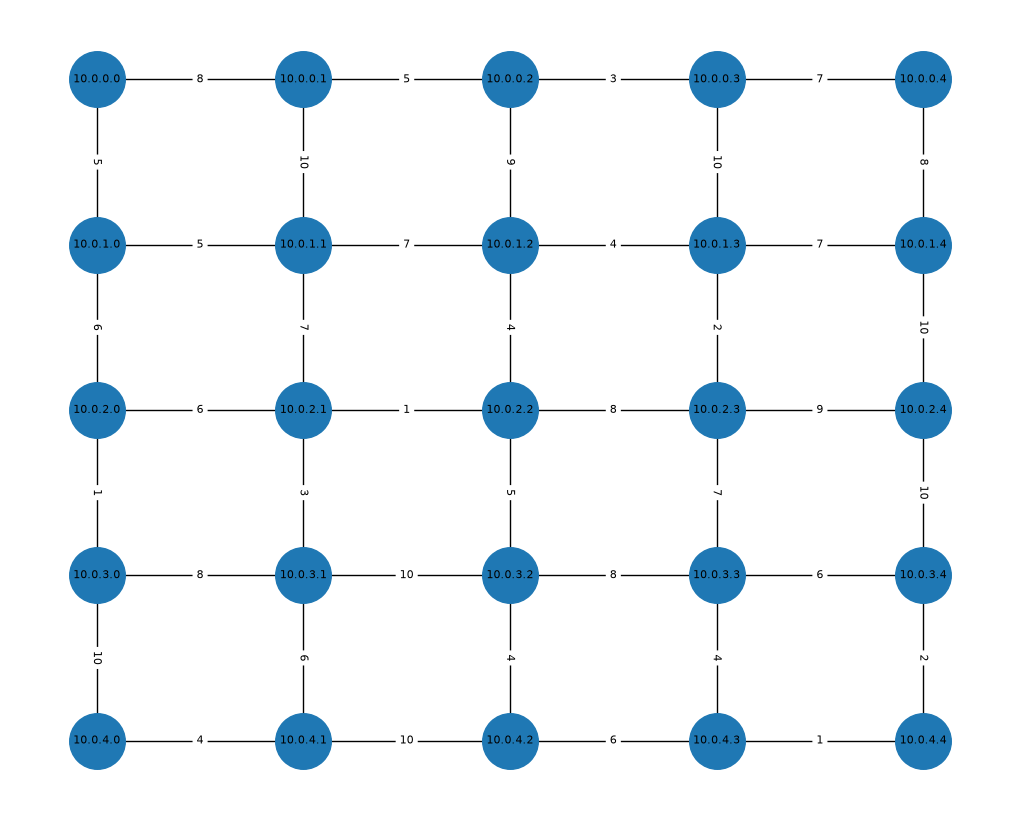
\includegraphics[width=\textwidth]{figures/initial_topology.png}
  \caption{Початкова топологія мережі}
  \label{fig:initial-topology}
\end{figure}

Після видалення 6 ребер результуючий граф містить 34 ребра. Перевірка за
допомогою функції \texttt{nx.is\_connected} повернула \texttt{True}, отже граф
залишився зв'язним. Результуючу топологію наведено на
рис.~\ref{fig:result-topology}.

\begin{figure}[H]
  \centering
  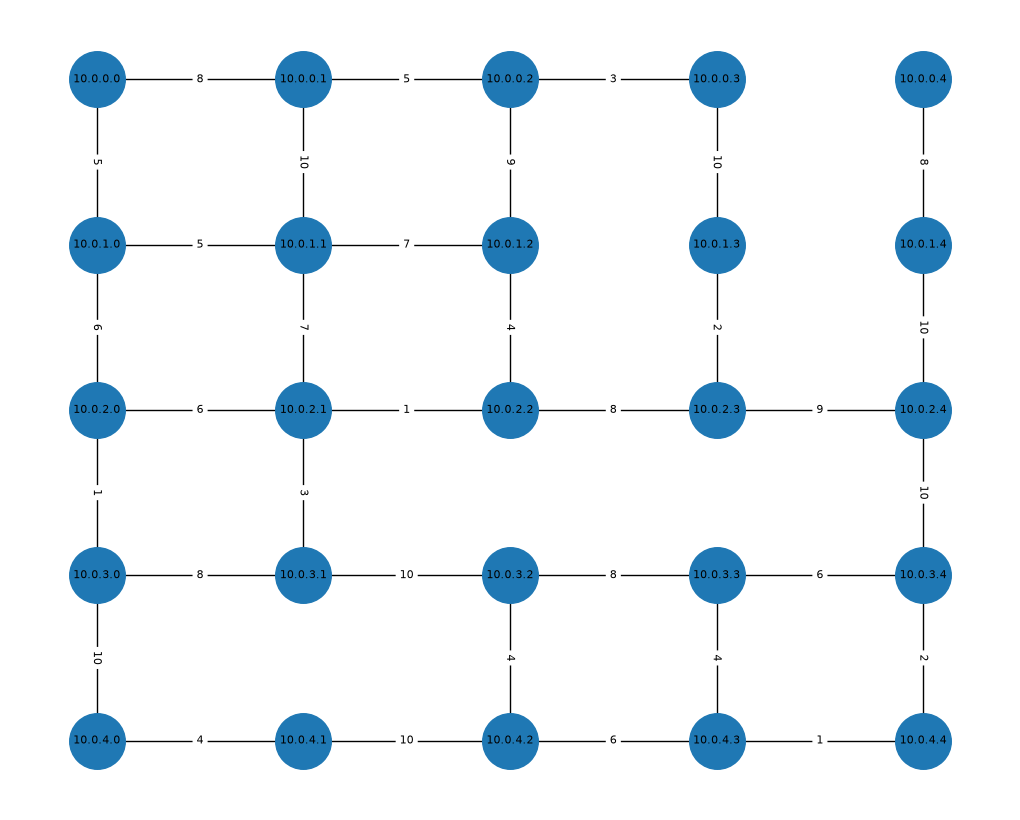
\includegraphics[width=\textwidth]{figures/resulting_topology.png}
  \caption{Топологія мережі після видалення шести ребер}
  \label{fig:result-topology}
\end{figure}

Отримані показники виконання наведено в табл.~\ref{tab:results}.

\begin{table}[H]
  \centering
  \renewcommand{\arraystretch}{1.18}
  \begin{tabular}{|l|c|}
    \hline
    \textbf{Показник} & \textbf{Результат} \\
    \hline
    Початкова кількість вузлів & 25 \\ \hline
    Початкова кількість ребер & 40 \\ \hline
    Кількість видалених ребер & 6 \\ \hline
    Кількість ребер після видалення & 34 \\ \hline
    Зв'язність результуючого графа & Так \\ \hline
  \end{tabular}
  \caption{Результати виконання}
  \label{tab:results}
\end{table}

\section{Висновок}

У лабораторній роботі згенеровано зважений неорієнтований граф із топологією
квадратної решітки. Вузли отримали унікальні адреси відповідно до їхньої
позиції, а канали зв'язку подано зваженими ребрами. Випадкові ваги ребер
моделювали затримку в заданому діапазоні. Із графа видалено шість ребер зі
збереженням його зв'язності. Бібліотеку NetworkX використано для подання та
перевірки графа, matplotlib --- для візуалізації, а Jupyter Notebook --- для
поєднання програмного коду, пояснень і результатів виконання.

\end{document}
